\begin{problem}{1}
    Use the following method to derive the integration formula:
    \begin{equation}
        \int_{0}^{\infty} e^{-x^{2}}\cos(2bx)dx = \frac{\sqrt{2}}{\pi}e^{-b^{2}} \quad (b>0)
    \end{equation}
    \begin{enumerate}
        \item Show that the sum of the integrals of $e^{-z^{2}}$ along the lower and upper horizontal legs of the rectangular path in the figure:\\
        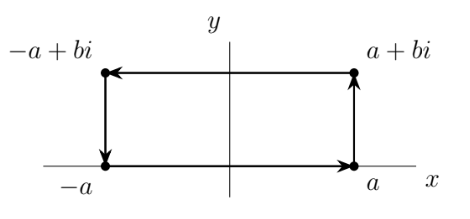
\includegraphics[width = 0.4\textwidth]{imgs/P1.png}\newline   
        can be written as:
        \vspace{-0.5cm}
        \begin{equation}
            2\int_{0}^{a}e^{-x^{2}} dx - 2e^{b^{2}}\int_{0}^{a}e^{-x^{2}}\cos(2bx)dx
        \end{equation}
        and that the sum of the integrals along the vertical legs on the right and left can be
written as:
        \begin{equation}
            ie^{-a^{2}}\int_{0}^{b}e^{y^{2}-i2ay}dy - ie^{-a^{2}}\int_{0}^{b}e^{y^{2}+i2ay}dy   
        \end{equation}
        Thus, with the aid of the Cauchy-Goursat theorem, show that:
        \begin{equation}
            \int_{0}^{a}e^{-x^{2}}\cos(2bx)dx = e^{-b^{2}}\int_{0}^{a}e^{-x^{2}}dx + e^{-(a+b^{2})}\int_{0}^{a}e^{y^{2}}\sin(2ay)dy
        \end{equation}

        \item By accepting the fact that:
        \begin{equation}
            \label{eq:P1-1}\int_{0}^{\infty}e^{-x^{2}}dx = \frac{\sqrt{\pi}}{2}
        \end{equation}
        and observing that:
        \begin{equation}
            \left|\int_{0}^{a}e^{y^{2}}\sin(2ay)dy\right| \leq \int_{0}^{a}e^{y^{2}}dy
        \end{equation}
        obtain the desired integration formula by letting a tend to infinity in the equation at the end of part (a).
    \end{enumerate}
\end{problem}
\subsection*{Solución}
El teorema de Cauchy-Goursat nos indica que la integral sobre la función $f$ que es analítica para todos los puntos contenidos en $C$, será cero. Esto hace necesario comprobar que la función $f(z) = e^{-z^{2}}$ es analítica en este contorno, debido a que esta función no tiene ninguna singularidad dentro de $C$ entonces se dice que es analítica en $C$. 

\begin{gather}
    \oint e^{z^{2}}dz = 0
\end{gather}
la parametrización indicada para esta función implica que para los caminos horizontales $z_1 = x + i0 \quad dz_1 = dx$ y $z_2 = x + ib \quad dz_2 = dx$, entonces, para estos caminos la integral será:

\begin{gather*}
    C_1 + C_2 = \int_{-a}^{a}e^{-x^2}dx + \int_{a}^{-a}e^{-(x + ib)^2}dx = 2\int_{0}^{a}e^{-x^2}dx - 2e^{b^2}\int_{0}^{a}e^{-x^2}e^{- i2xb}dx
\end{gather*}
usando el teorema de De Moivre, para expresar exponenciales con potencias imaginarias en términos de senos y cosenos se obtiene.

\begin{gather*}
    C_1 + C_2 = 2\int_{0}^{a}e^{-x^2}dx - 2e^{b^2}\int_{0}^{a}e^{-x^2}\left(\cos(2xb) - i\sin(2xb)\right)dx
\end{gather*}
como la función seno tiene simetría impar, entonces en el intervalo de ($-a,a$) su integral será cero. 
\begin{gather}
    C_1 + C_2 = 2\int_{0}^{a}e^{-x^2}dx - 2e^{b^2}\int_{0}^{a}e^{-x^2}\cos(2xb)dx
\end{gather}
Ahora, para los caminos con orientación vertical, las parametrizaciones nos indican que $z_3 = a + iy, \quad dz_3 = idy$ y $z_4 = -a + iy \quad dz_4 = idy$, remplazando.

\begin{gather}
    C_3 + C_4 = \int_{0}^{b}e^{-(a + iy)^2}idy + \int_{b}^{0}e^{-(-a + iy)^2}idy = e^{-a^2}\int_{0}^{b}e^{y^2 - i2ay}idy - e^{-a^2}\int_{0}^{b}e^{y^2 + i2ay}idy
\end{gather}
El teorema de Cauchy-Goursat nos dice que la suma de estas cuatro integrales debe ser cero

\begin{gather*}
    2\int_{0}^{a}e^{-x^2}dx - 2e^{b^2}\int_{0}^{a}e^{-x^2}\cos(2xb)dx +ie^{-a^2}\int_{0}^{b}e^{y^2 - i2ay}dy - ie^{-a^2}\int_{0}^{b}e^{y^2 + i2ay}dy = 0\\ 
    2\int_{0}^{a}e^{-x^2}dx +ie^{-a^2}\int_{0}^{b}e^{y^2}e^{-i2ay}dy =  2e^{b^2}\int_{0}^{a}e^{-x^2}\cos(2xb)dx  + ie^{-a^2}\int_{0}^{b}e^{y^2}e^{i2ay}dy
\end{gather*}
Expresando los términos exponenciales con potencias imaginarias en términos de funciones trigonométricas, sumando y cancelando términos semejantes se obtiene:

\begin{gather*}
    2e^{b^2}\int_{0}^{a}e^{-x^2}\cos(2xb)dx = 2\int_{0}^{a}e^{-x^2}dx +  2e^{-a^2}\int_{0}^{b}e^{y^2}\sin(2ay)dy  \\
    \int_{0}^{a}e^{-x^2}\cos(2xb)dx = e^{-b^2}\int_{0}^{a}e^{-x^2}dx +  e^{-(a^2 + b^2)}\int_{0}^{b}e^{y^2}\sin(2ay)dy
\end{gather*}
cuando $a \rightarrow \infty$ se obtiene 

\begin{gather*}
    \int_{0}^{\infty}e^{-x^2}\cos(2xb)dx = e^{-b^2}\int_{0}^{\infty}e^{-x^2}dx +  \lim_{a\rightarrow\infty}e^{-(a^2 + b^2)}\int_{0}^{b}e^{y^2}\sin(2ay)dy
\end{gather*}
analizando el segundo término del lado derecho la expresión

\begin{gather*}
    \lim_{a\rightarrow\infty}e^{-(a^2 + b^2)}\int_{0}^{b}e^{y^2}\sin(2ay)dy = \cancelto{0}{\lim_{a\rightarrow\infty}e^{-(a^2 + b^2)}} \quad \left(\lim_{a\rightarrow\infty} \int_{0}^{b} e^{y^2}\sin(2ay)dy\right) = 0
\end{gather*}
la integral del término del lado derecho esta dada por (\ref*{eq:P1-1}), esto implica

\begin{mdframed}
    \vspace{-0.5cm}
    \begin{gather}
        \int_{0}^{\infty}e^{-x^2}\cos(2xb)dx = e^{-b^2}\frac{\sqrt{\pi}}{2}
    \end{gather}
\end{mdframed}